% !TEX root = master.tex
\begin{flushleft}
	%\vspace*{0.5cm} 
%\textbf{\LARGE Bewertung potenzieller Risiken}
%\vspace*{0.1cm}
\end{flushleft}

\chapter{Risikomanagement}
\label{chapt:Risikomanagement}
%Erstellt zu eurem Projekt eine Risikoanalyse und betrachtet die Kernrisiken (mind.
%3 Stück) im Detail:
%– Klassifizierung nach Eintrittswahrscheinlichkeit und Auswirkung
%– Erstellung einer geeigneten Visualisierung
%– Beschreibung der Auswirkung auf die Projektdimensionen (-> Risikotyp)
%– Entwicklung geeigneter Maßnahmen und Einordnung in die Maßnahmen-Kategorien
%– Begründung von o.g. Elementen
\label{chapter:6}
\section{Bewertung potenzieller Risiken}
%\textbf{\LARGE Bewertung potenzieller Risiken}
%\vspace*{0.1cm}

Im Rahmen des Risikomanagements wurden 23 potenzielle Risiken identifiziert. Wie diese hinsichtlich ihrer Eintrittswahrscheinlichkeiten und Auswirkungen zu bewerten sind, ist in Abbildung \ref{fig:risikomatrix} visualisiert. Die Zahlen innerhalb der Quadrate entsprechen den Identifikationsnummern der verschiedenen Risiken, welche in Tabelle \ref{tab:risikotb} ausformuliert sind. Der Risikowert ergibt sich aus dem Produkt der Eintrittswahrscheinlichkeit (WSK) und Stärke eines Risikos. 

\begin{figure}[h]
	\centering
	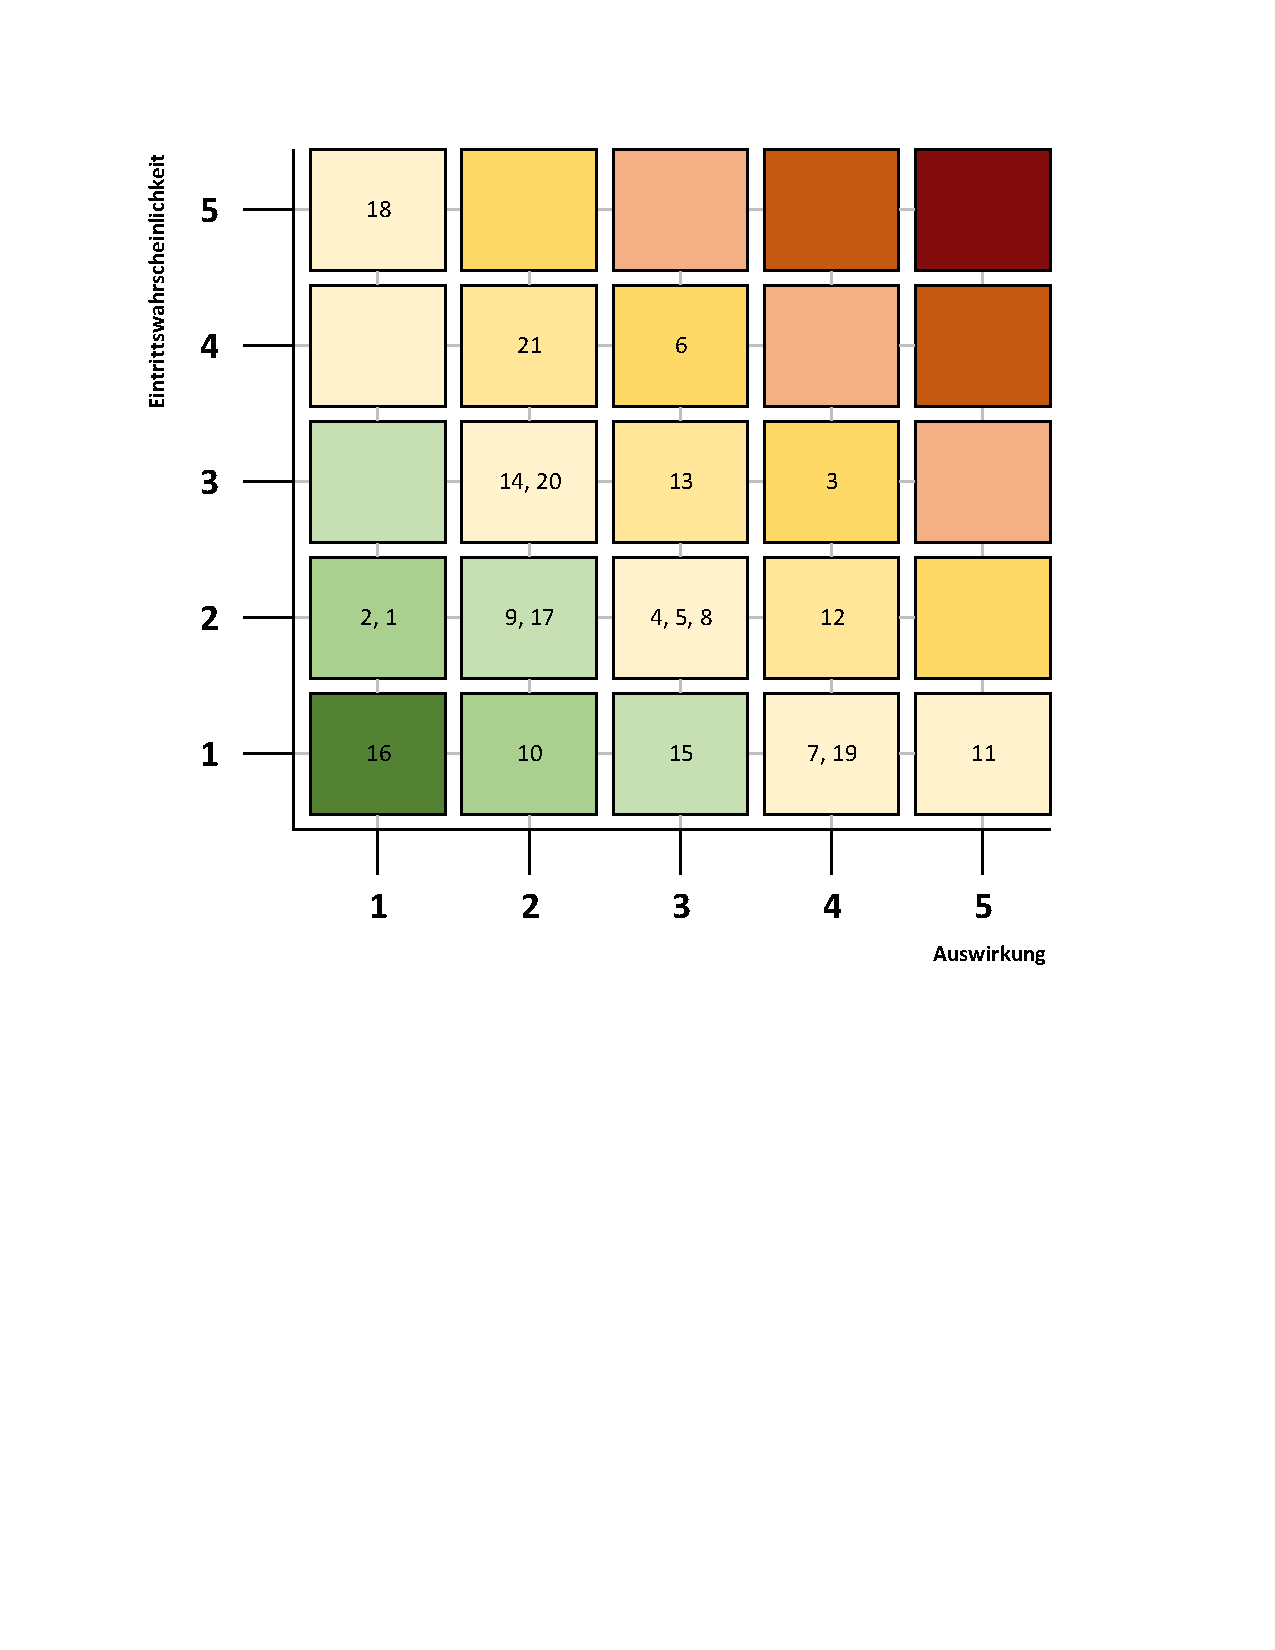
\includegraphics[width=0.85\linewidth]{img/Risikomatrix}
	\caption{Risikomatrix}
	\label{fig:risikomatrix}
\end{figure}


\footnotesize
\newcolumntype{P}[1]{>{\raggedright\arraybackslash}p{#1}}
\newgeometry{left=1cm,right=1cm,top=1cm,bottom=1cm}
\begin{landscape}
	\pagestyle{headings}
	\pagestyle{empty}
	\begin{longtable}{| P{0.5cm} | P{1.7cm} | P{3cm} | P{5cm} | P{1cm} | P{1cm} | P{1cm} | P{2.2cm} | P{2cm} | P{5cm} |}
		
	\hline
	\textbf{ID} &\textbf{Risikotyp}&\textbf{Titel} &\textbf{Beschreibung} &\textbf{WSK} &\textbf{Stärke} &\textbf{Risiko} &\textbf{Problem-Zeitpunkt} &\textbf{Maßnahmen-Kategorie} &\textbf{Maßnahme}\\
	\hline
	\endfirsthead
		
	\multicolumn{10}{c}%
	{\tablename\ \thetable\ -- \textit{Fortsetzung von vorheriger Seite}} \\
	\hline
	\textbf{ID} &\textbf{Risikotyp}&\textbf{Titel} &\textbf{Beschreibung} &\textbf{WSK} &\textbf{Stärke} &\textbf{Risiko} &\textbf{Problem Zeitpunkt} &\textbf{MKategorie} &\textbf{Maßnahme}\\
	\hline
	\endhead
		
	\multicolumn{10}{r}
	{\textit{Weiter auf nächster Seite}} \\
	\endfoot
	\endlastfoot
	
	1&Zeit&Technologie-verschlossenheit&Diffuse Angst vor Veränderungen führt zu fehlender Akzeptanz der Lösung bei den Nutzern&2&1&2&Nach Projektabschluss&Verringern&
	1. Kommunikations- und Schulungsprogramme, um Mitarbeiter über die Vorteile der Digitalisierung aufzuklären und ihre Ängste zu mildern.\\
	\hline

	2&Zeit&Angst vor Arbeitsplatzverlust&Arbeitsplatzverlust (v.a. nach kürzlichem Downsizing) führt zu Widerstand bei Poststellenmitarbeitern&2&1&2&Kickoff bis nach Projektabschluss&Übernehmen&
	1. Regelmäßige Überprüfung des Stimmungsbildes\\
	\hline
	
	3&Leistung&Vernachlässigung der Mitarbeiter-anforderung&Missachtung der Wünsche und Anforderungen der Sachbearbeiter führt zu fehlender Akzeptanz der Lösung&3&4&12&Nach Projektabschluss&Verringern&
	1. Einbeziehung der Mitarbeiter in Planung\newline
	2. Regelmäßige Feedbackschleifen während der Entwicklungsphase\\ 
	\hline

	4&Leistung&Vernachlässigung Kundenanforderung&Missachtung der Wünsche und Anforderungen von Kunden führt zu fehlender Akzeptanz der Lösung&2&3&6&Nach Projektabschluss&Verringern&
	1. Einbeziehung der Kunden in Planung\newline
	2. Regelmäßige Feedbackschleifen während der Entwicklungsphase\\ 
	\hline

	5&Zeit&Fachkräftemangel&Mangelnde Fachkräfte für die Entwicklung bei CP Service GmbH führt zu Ressourcenüberschreitung&2&3&6&Kickoff bis Projektabschluss&Verringern&
	1. Einstellung neuer Mitarbeiter\newline
	2. Weiterbildung bestehender Mitarbeiter\newline
	3. Einbindung externer Berater\\ 
	\hline
	
	6&Zeit&Softwarefehler in Pilotierung&Pilotierung mit fehlerhaftem Produkt führt zu zusätzlichem Entwicklungsaufwand und Missgunst bei Großkunden&4&3&12&Pilotierung&Verringern&
	1. Durchführung gründlicher Tests vor der Pilotierung\newline
	2. Implementierung robuster Unit-, Integrations- und End-to-End-Tests\\
	\hline
	
	7&Kosten&Datenleak&Mangelnder Informationssicherheit führt zu Datenleaks und Strafzahlungen während Pilotierung&1&4&4&Pilotierung&Verringern&
	1. Datenschutzbeauftragten einbinden\newline
	2. Informationssicherheitskonzept erstellen\\ 
	\hline
	
	8&Zeit&Unterschätzung Entwicklungs-aufwand&Unterschätzung des Entwicklungsaufwandes führt zu Ressourcenüberschreitung&2&3&6&Entwicklung bis Pilotierung&Verringern&
	1. Planning Poker mit möglichst allen Projektmitgliedern\newline
	2. Hinreichende Puffer einplanen\\ 
	\hline
		
	9&Leistung&Unklarheit Rollenverteilung&Unklarer Rollendefinitionen führen zu Verantwortungsdiffusion und mangelnder Produktqualität&2&2&4&Entwicklung bis Pilotierung&Verringern&
	1. Klare Rollendefinition mit Kompetenzen\newline
	2. Verantwortung und Aufgaben\\ 
	\hline
	
	10&Zeit&Trotzreaktion&Top-Down-Managementstil und Einmischung in den operativen Betrieb durch die Geschäftsführung führt zu fehlender Akzeptanz bei Mitarbeitern&1&2&2&Nach Projektabschluss&Übernehmen&
	1. Stimmungslage im Blick behalten\\ 
	\hline
	
	11&Leistung&Strategiewechsel&Interner Strategiewechsel führt zu Verlust des Supports vom Top-Management&1&5&5&Kickoff bis Projektabschluss&Übernehmen&
	1. Regelmäßige Überprüfung des Supports durch Top-Management\\ 
	\hline
	
	12&Zeit&Absage Pilotierung&Angst fehlerhaftem Produkt führt dazu, dass die Großkunden nicht an der Pilotierung teilnehmen möchten&2&4&8&Pilotierung&Verringern&
	1. Verhandlung der verbindlichen Teilnahme im Voraus\newline
	2. Übernahme der durch Fehler entstehenden Schäden\\ 
	\hline
		
	13&Zeit&Disharmonie im Team&Fehlende Harmonie (Streit) im Team führt zu längerer Projektlaufzeit&3&3&9&Kickoff bis Projektabschluss&Verringern&
	1. Regelmäßige Retrospektiven\newline
	2. Teambuilding-Maßnahmen\newline
	3. Team-Konstellation konstant halten und Vermittlung während der Storming-Phase\newline
	4. Personenspezifische Maßnahmen zwecks Minimierung des Konfliktpotenzials\\ 
	\hline
	
	14&Zeit&Technische Schwierigkeiten&Technische Schwierigkeiten bei der Entwicklung führen zu Ressourcenüberschreitung&3&2&6&Entwicklung&Verringern&
	1. Externe Hilfe auf Abruf bereithalten\newline
	2. Angemessene Puffer\\
	\hline
	
	15&Zeit&Gesetzesänderung&Veränderte gesetzliche oder regulatorische Vorgaben führen zu Anpassungsbedarf bei Lösung&1&3&3&Kickoff bis Projektabschluss&Übernehmen&
	1. Gesetzeslage im Blick behalten\\ 
	\hline
	
	16&Leistung&Technologie-ablösung&Technologische Innovation führt dazu, dass Lösung bis zum Projektabschluss bereits veraltet ist&1&1&1&Kickoff bis Projektabschluss&Übernehmen&
	1. Technische Entwicklung im Blick behalten\\
	\hline
	
	17&Leistung&Präferenz Papierschnittstelle&Bevorzugung der herkömmlichen Papierschnittstelle führt zu Ablehnung der Lösung bei C- und B-Kunden&2&2&4&Nach Projektabschluss&Übernehmen& 
	1. Intensive Kommunikation der Vorteile\newline
	2. Parallelbetrieb des digitalen und des papierbasierten Prozesses\newline
	3. Verpflichtung zum neuen Prozess\newline
	4. Inkaufnahme von Kündigungen\\ 
	\hline
	
	18&Zeit&Personalausfall&Unvorhergesehener Vorfall (z.B. Krankheit) führt zu Ausfall von Personal&5&1&5&Kickoff bis Projektabschluss&Verringern&
	1. Einplanung ausreichender Puffer\newline
	2. Rechnung mit realistischen Annahmen\\ 
	\hline

	19&Kosten&Softwarefehler in  Rollout&Mangelhaftes Controlling führt zu Rollout mit fehlerhaftem Produkt und Verlust von Kunden&1&4&4&Rollout&Verringern&
	1. Intensives Controlling\newline
	2. Intensives Testing vor Rollout\\ 
	\hline
	
	20&Zeit&Mangelhafte Dokumentation&Mangelhafte Produktdokumentation führt zu eingeschränkten Wartbarkeit und Weiterentwicklung der Lösung nach Projektabschluss&3&2&6&Nach Projektabschluss&Verringern&
	1. Intensives Controlling der Anfertigung der Produktdokumentation\\ 
	\hline
	
	21&Kosten&Transatlantischer Neid&Ausschluss internationaler Kunden vom Rollout führt zu deren Unzufriedenheit/Kündigung aufgrund ungleicher Behandlung&4&2&8&Kickoff bis nach Projektabschluss&Übernehmen&
	1. Stimmungslage im Blick behalten\\ 
	\hline
	

\end{longtable}
\captionof{table}{Risikotabelle} \label{tab:risikotb}
\end{landscape}
\pagestyle{headings}
\restoregeometry
\normalsize

% ----------------
\section{Detailbetrachtung der Kernrisiken}
%\textbf{\LARGE Detailbetrachtung der Kernrisiken}
%\vspace*{0.1cm}

Aufgrund des hohen Zeitdrucks scheint es vertretbar, im Rahmen des Risikomanagements eine Vorauswahl zu treffen. So werden im folgenden nur jene Risiken analysiert, deren Risikowert größer als 7 ist. Die restlichen Eventualitäten werden aufgrund einer geringen Eintrittswahrscheinlichkeit und/oder Stärke zugunsten eines zügigen Projektfortschritts vernachlässigt. Die drohende Insolvenz durch die Kündigung der Großkunden resultiert somit in einer erzwungenen Risikoaffinität bei der CP Service GmbH.


% ---------------- 1 KernRisiko

\vspace*{0.3cm}
\textbf{Risiko 13 - Disharmonie im Team}
\vspace*{0.1cm}

\begin{wrapfigure}{l}{0.15\textwidth}
	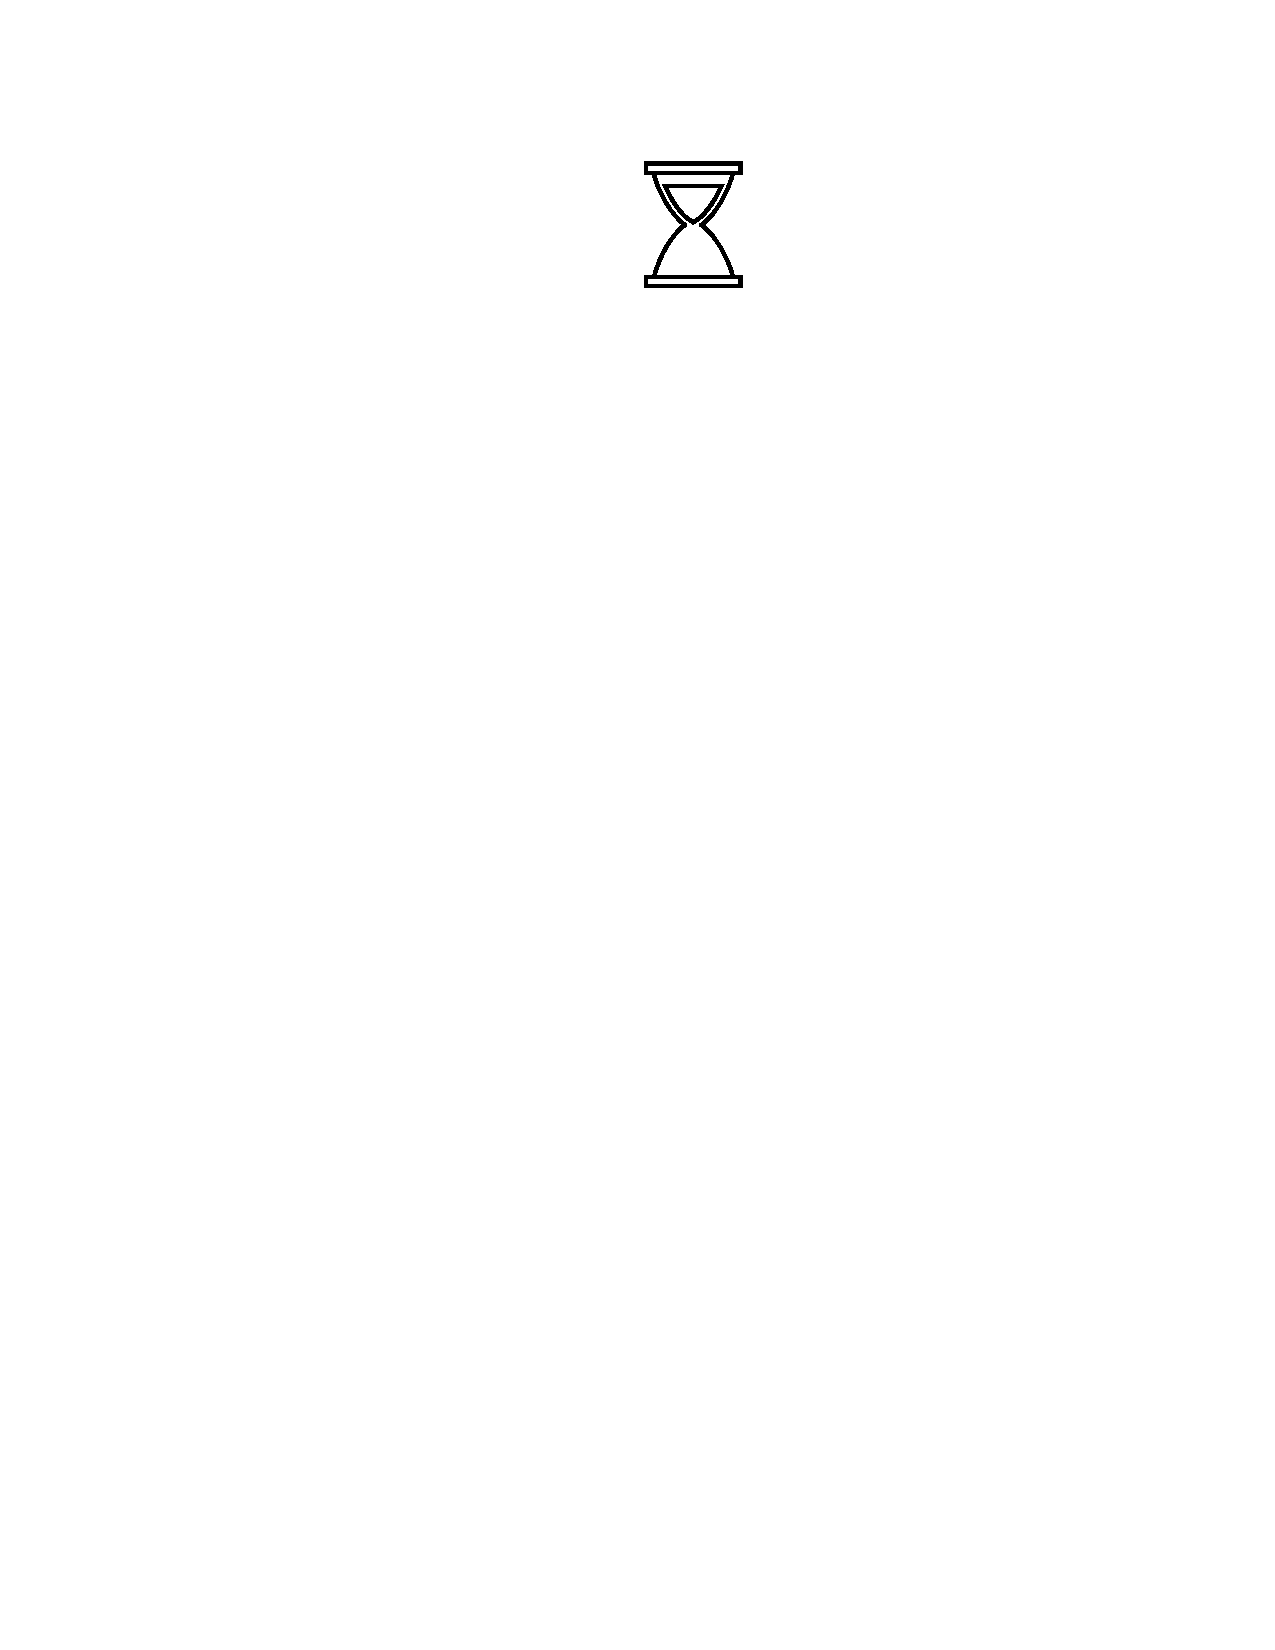
\includegraphics[width=\linewidth]{img/Risikotyp_Zeit}
\end{wrapfigure}

Die Team-Konstellation birgt ein nicht zu vernachlässigendes Konfliktpotenzial. Zunächst gilt es festzustellen, dass der Product Owner Franz Urlaub recht unerfahren und darüber hinaus unbeliebt bei der Belegschaft ist. Dies könnte dazu führen, dass die Team-Mitglieder ihm weniger Respekt entgegenbringen und seine Anweisungen missachten. Sollte es zudem Streit unter den Projektmitgliedern geben, würde Franz Urlaub aufgrund seines Laissez-Faire-Führungsstils nicht eingreifen, was zu einer Eskalation des Konflikt führen könnte. Auch die beiden Scrum-Master könnten in diesem Fall nur bedingt vermitteln, da sie jeweils nur zu 50\% im Projekt involviert sind. Somit fehlt dem Team eine verlässliche zentrale Anlaufstelle, welche die Stimmung einfangen und Auseinandersetzungen präventiv entgegenwirken kann. Konflikte können prinzipiell jederzeit entstehen, im Kontext dieses Projekts sind jedoch zwei Szenarien besonders wahrscheinlich. Zum einen könnte es Streit zwischen Tom Schulze und Harry Mayer geben, weil Tom Wert auf Wissensmanagement und Erfahrungsaustausch legt, während Harry Mayer lieber isoliert für sich arbeitet. Ein weiterer potenzieller Reibungspunkt sind die Unterschiede im Engagement zwischen Stefan Schmitt und Maria Musterfrau. Stefan möchte zukünftig gerne auf eine Teilzeitposition reduzieren, um mehr Zeit mit seiner Familie verbringen zu können, während Maria hoch-engagiert und sehr ehrgeizig am Projekt partizipiert. Der Unterschied in den Prioritäten der beiden Parteien könnte einen Streit auslösen. Sollte Stefan Schmitt noch während des Projekts auf eine Teilzeitstelle wechseln, würde sich das Konfliktpotenzial außerdem insgesamt erhöhen, da die anderen Projektmitglieder seinen Workload übernehmen müssten, was zu Stress und Überlastung führen könnte. Das Risiko lässt sich zwar nicht gänzlich vermeiden, dessen Eintrittswahrscheinlichkeit kann jedoch über die folgenden Maßnahmen reduziert werden:
\begin{itemize}
	\item Zu Beginn der Entwicklungsphase wird von den Scrum-Mastern ein Team-Building-Event durchgeführt, um den Gruppenzusammenhalt zu stärken und die Storming-Phase nach Tuckman zu beschleunigen
	\item Der Product Owner handelt mit Stefan Schmitts Führungsperson noch vor Projektbeginn aus, dass dieser dem Team bis Projektabschluss in Vollzeit erhalten bleibt.
	\item Der Product Owner stellt sicher, dass nicht aus Gründen der Zeitersparnis auf die Retrospektiven am Ende der Sprints verzichtet wird.
\end{itemize}


% ---------------- 2 KernRisiko

\vspace*{0.3cm}
\textbf{Risiko 3 - Vernachlässigung der Mitarbeiteranforderungen}
\vspace*{0.1cm}

\begin{wrapfigure}{l}{0.15\textwidth}
	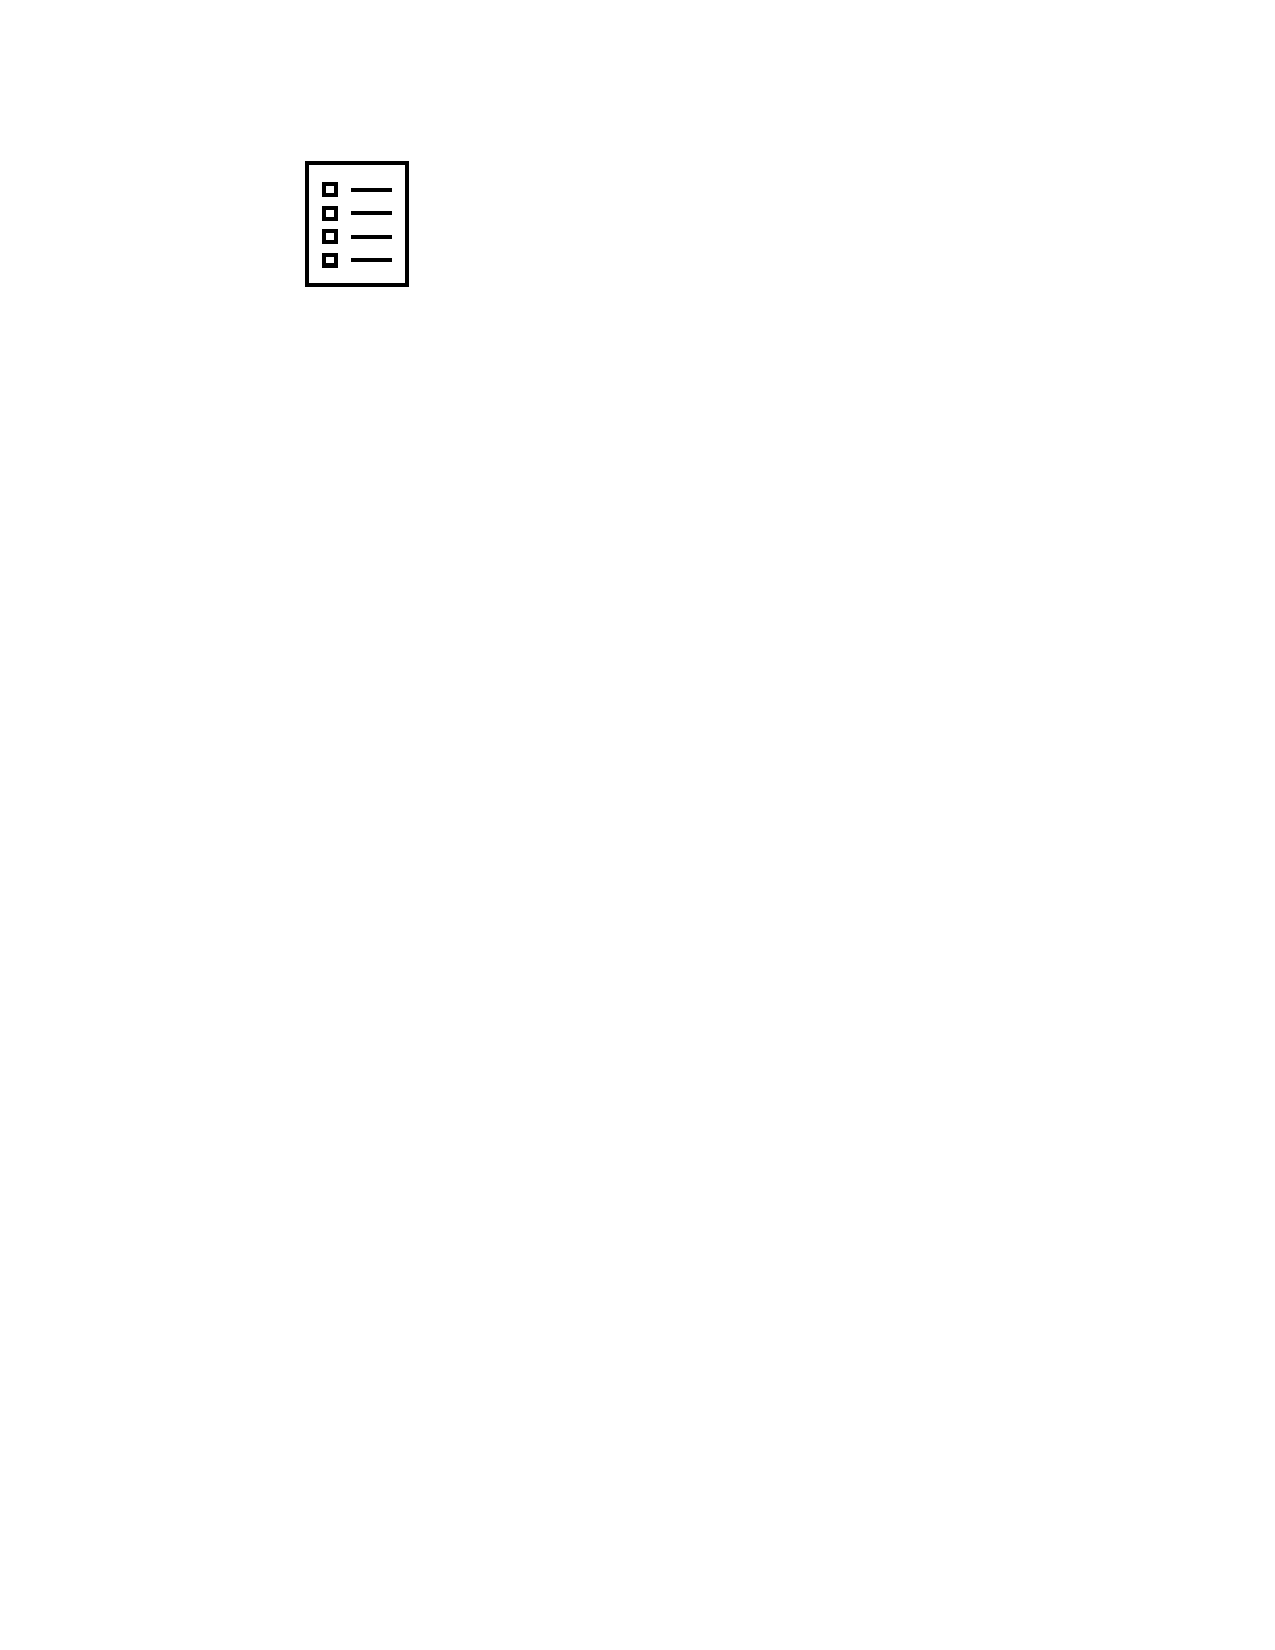
\includegraphics[width=\linewidth]{img/Risikotyp_Leistung}
\end{wrapfigure}

Aufgrund der Tatsachen, dass die Geschäftsführung die Kundenzufriedenheit über das Wohl der Mitarbeiter stellt und das Projekt unter großem Zeitdruck durchgeführt wird, ist es wahrscheinlich, dass die Wünsche der Mitarbeiter bei der Konzipierung der digitalen Schnittstelle nicht ausreichend berücksichtigt werden. Dies wäre fatal, da es schon jetzt regelmäßige Beschwerden von Seiten der Sachbearbeiter gibt. Wenn diese nicht in den Entwicklungsprozess eingebunden werden und das Ergebnis des Projekts eine Software-Lösung ist, die nur die Bedürfnisse der Kunden, nicht aber die der internen Nutzer, adressiert, kann dies zu Frust und Ablehnung in der Belegschaft führen. In Kombination mit dem autoritären Top-Down Managementstil der Geschäftsführung und einer gewissen Grundverstimmtheit aufgrund starker Stellenkürzungen innerhalb der letzten drei Jahre, könnte dies eine betriebsschädigende Abwehrhaltung auf Seiten der Arbeitnehmer hervorrufen. Diese Unzufriedenheit könnte sich in der Nicht-Verwendung des neuen Systems und dem Festhalten an alten Prozessen sowie einer langsamen Auftragsabarbeitung oder einer Arbeitsverweigerung manifestieren. Auch wenn die Lösung inhaltlich und qualitativ den in der Planung festgelegte Anforderungen entspricht, lässt sich argumentieren, dass sich ein Eintreten des Risikos dennoch auf die Projektdimension \textit{Leistung} auswirkt, da die Anforderungen der Mitarbeiter nicht enthalten und somit auch nicht erfüllt wurden. Um die Wahrscheinlichkeit für das Eintreten dieses Risikos zu verringern, werden folgende Maßnahmen ergriffen:
\begin{itemize}
	\item Alle Sachbearbeiter werden dazu eingeladen bei der Erstellung des Anforderungskatalogs im Rahmen der Projektplanung mitzuwirken und am Kickoff-Event teilzunehmen. Die Einladung erfolgt über den Product Owner und die Teilnahme ist freiwillig.
	\item Die Sachbearbeiter werden monatlich vom Product Owner per E-Mail über den Stand der Entwicklung informiert und können sich bei Rückfragen an ihn wenden. Dies erzeugt ein Gefühl der Teilhabe, wodurch die Akzeptanz des Endprodukts erhöht wird.
\end{itemize}


% ---------------- 3 KernRisiko

\vspace*{0.3cm}
\textbf{Risiko 12 - Absage Pilotierung}
\vspace*{0.1cm}

\begin{wrapfigure}{l}{0.15\textwidth}
	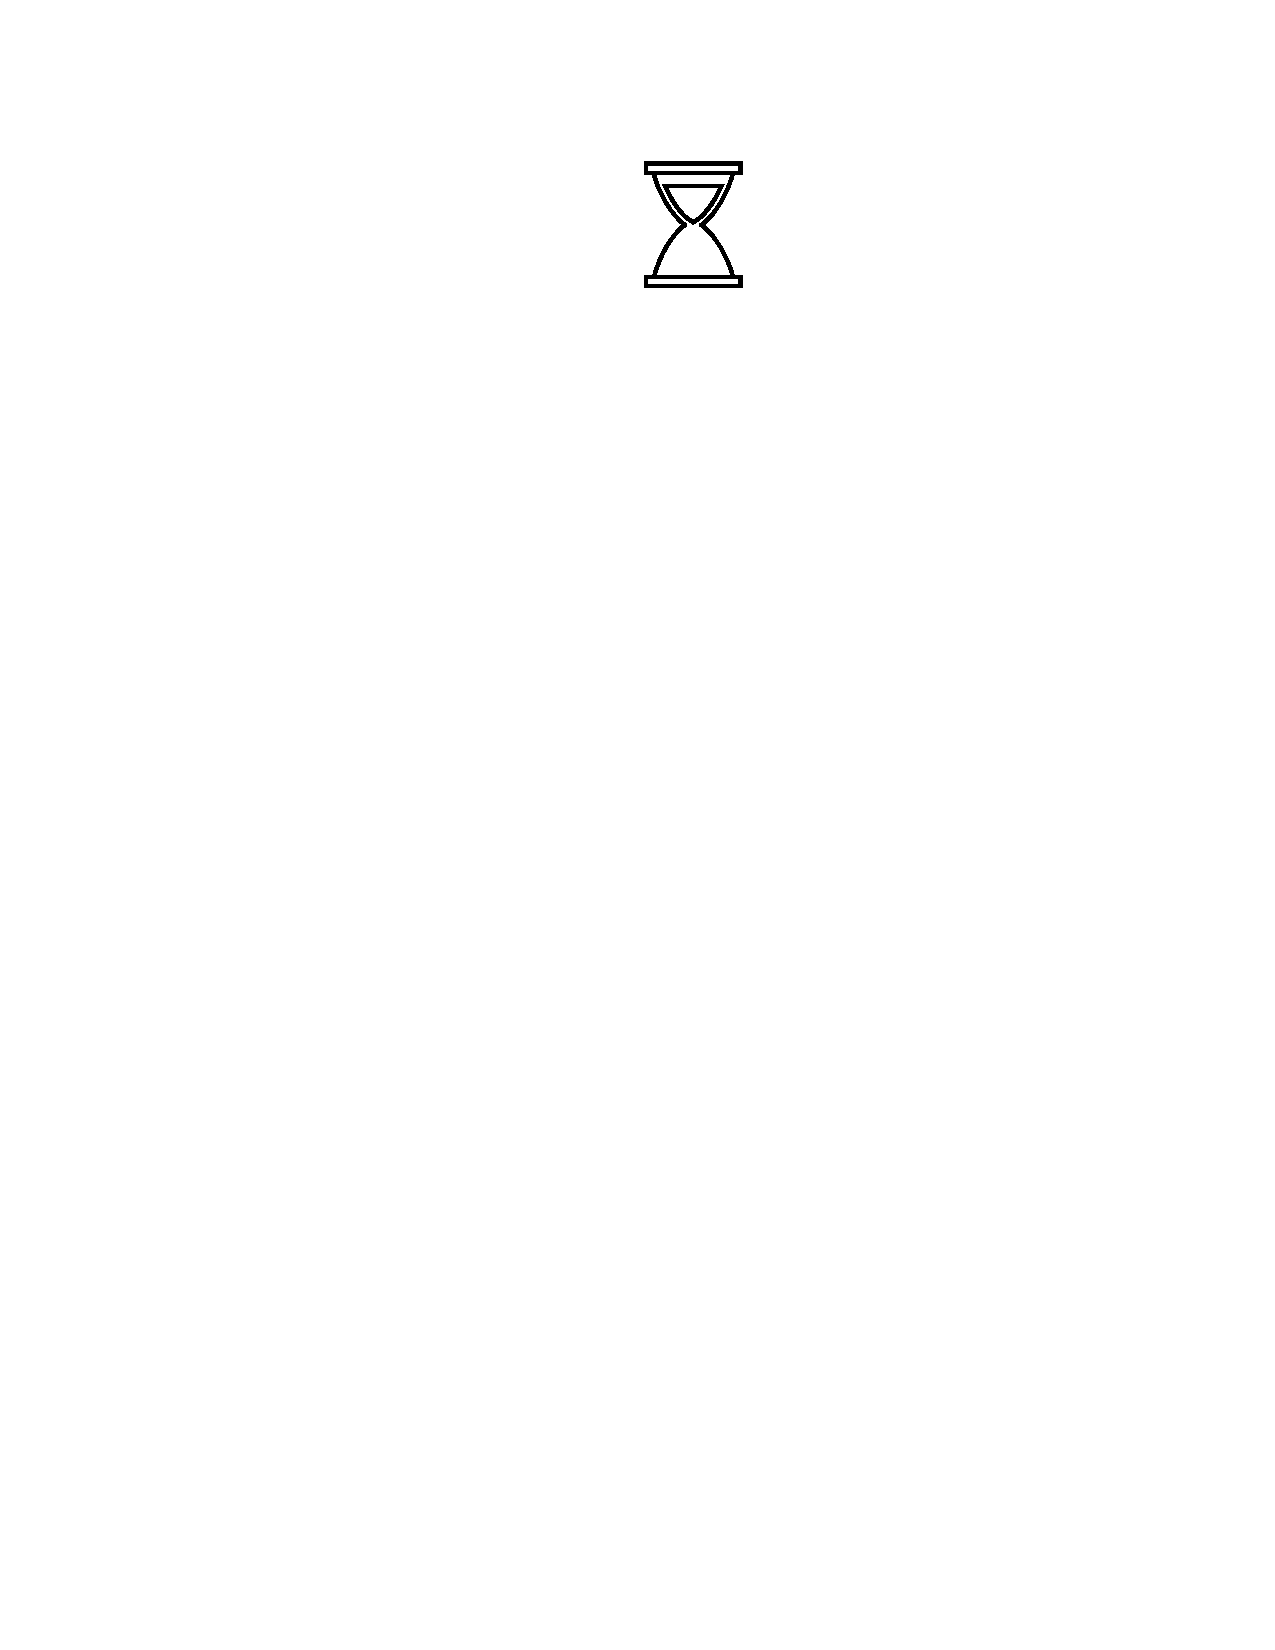
\includegraphics[width=\linewidth]{img/Risikotyp_Zeit}
\end{wrapfigure}

Die Idee hinter der Pilotierung ist es, den Großkunden so früh wie möglich die digitale Schnittstelle zur Verfügung zu stellen. Da beim erstmaligen Einsatz eines neuen Systems das Auftreten von Fehlern relativ wahrscheinlich ist, sind die Großkunden eventuell nicht bereit an der Pilot-Phase teilzunehmen. Stattdessen müsste die Pilotierung in Zusammenarbeit mit anderen Kunden erfolgen und die Großkunden würden erst bei der finalen Auslieferung Zugriff auf die Schnittstelle erhalten. Dies führt unweigerlich dazu, dass das Produkt nicht so gut auf die wichtigsten beiden Kunden maßgeschneidert werden kann und verlängert die Zeit bis diese das Produkt erhalten. Mit jeder verstreichenden Woche steigt jedoch die Gefahr, dass die Großkunden die Geduld verlieren und kündigen, da ihre Anliegen nicht schnell genug adressiert wurden. Als Risikotyp wurde die Projektdimension \textit{Zeit} gewählt, weil das oberste Ziel des Projektes die Abwendung der Insolvenz durch den Erhalt der Großkunden darstellt und die Auslieferung an selbige durch deren Verzicht auf die Pilotierung verzögert wird. Folgende Maßnahmen eignen sich, um die Eintrittswahrscheinlichkeit des Risikos zu minimieren:
\begin{itemize}
	\item Der Product Owner verhandelt mit den Großkunden zu Beginn der Planungsphase die Konditionen, welche erfüllt werden müssen, damit sie bereit sind an der Pilotierung teilzunehmen (z.B. 2-wöchiges Testing auf kundenähnlichem System im Vorlauf zur Pilot-Phase)
	\item Optional: Sollten die Sponsoren zustimmen, kann den Großkunden eine Übernahme der durch Bugs entstandenen Schäden angeboten werden.
\end{itemize}

% ---------------- 4 KernRisiko

\vspace*{0.3cm}
\textbf{Risiko 21 - Transatlantischer Neid}
\vspace*{0.1cm}

\begin{wrapfigure}{l}{0.15\textwidth}
	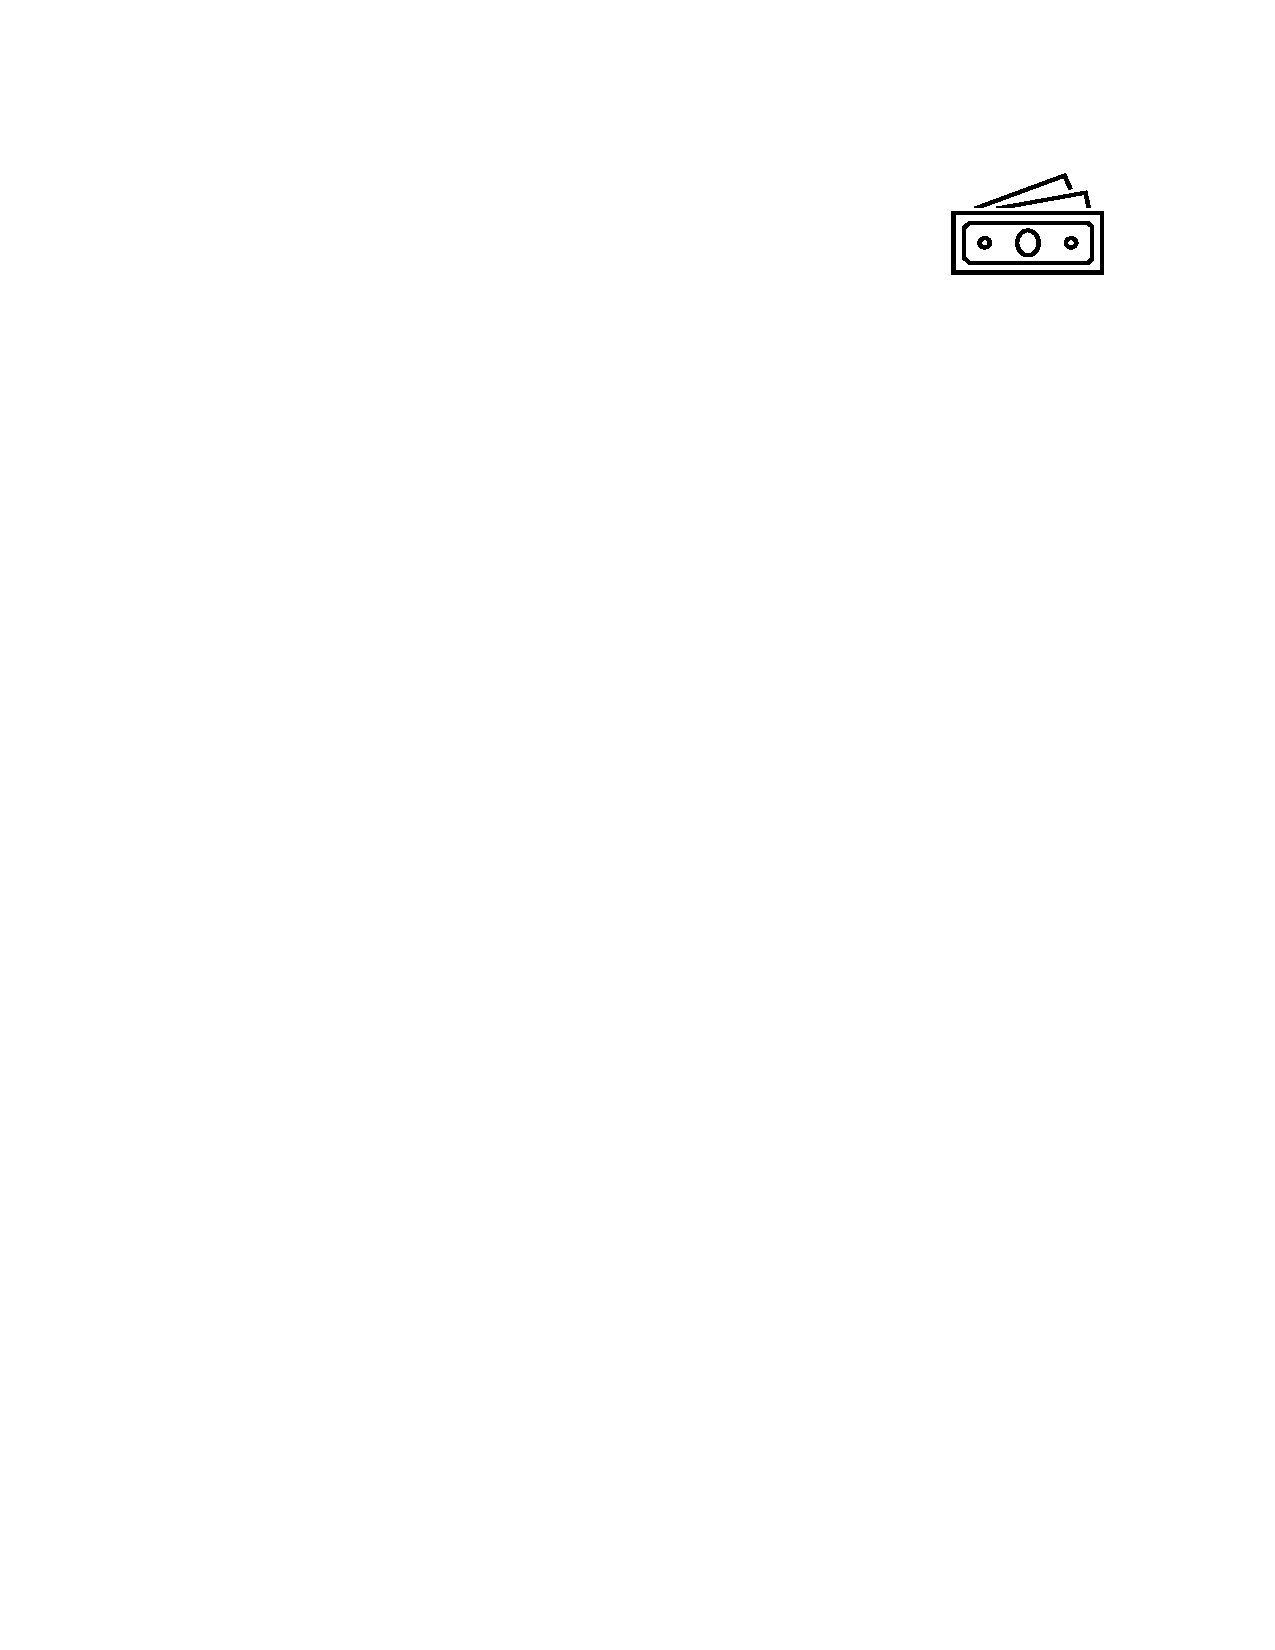
\includegraphics[width=\linewidth]{img/Risikotyp_Kosten}
\end{wrapfigure}

Wie zu Beginn klar definiert wurde, ist der Rollout ausschließlich auf deutsche Kunden begrenzt. Da die Digitalisierung der Schnittstelle jedoch eine signifikante Effizienzsteigerung auf Seiten der Kunden bedeutet und die Verzögerung bei der Abarbeitung von Aufträgen internationale Kunden aufgrund des langen Postweges besonders betrifft, ist es nicht unwahrscheinlich, dass diese zukünftig ebenfalls von der Softwarelösung profitieren wollen. Da es kaum gute Gründe gibt, die internationalen Kunden vom Rollout auszuschließen, wird diese Entscheidung auf Unverständnis stoßen. Dies verschlechtert nicht nur unser Verhältnis zu diesen Kunden, sonder könnte langfristig auch deren Kündigung führen. Dieses Risiko wird von der Projektleitung weder vermieden noch verringert, sondern in Kauf genommen. Folgende Maßnahmen sollten dennoch getroffen werden:

\begin{itemize}
	\item Der Product Owner kommuniziert regelmäßig mit den zuständigen Account Managern, um die Entwicklung der Stimmungslage unserer internationalen Kunden informiert zu sein. 
\end{itemize}


% ---------------- 5 KernRisiko

\vspace*{0.3cm}
\textbf{Risiko 6 - Softwarefehler in Pilotierung}
\vspace*{0.1cm}

\begin{wrapfigure}{l}{0.15\textwidth}
	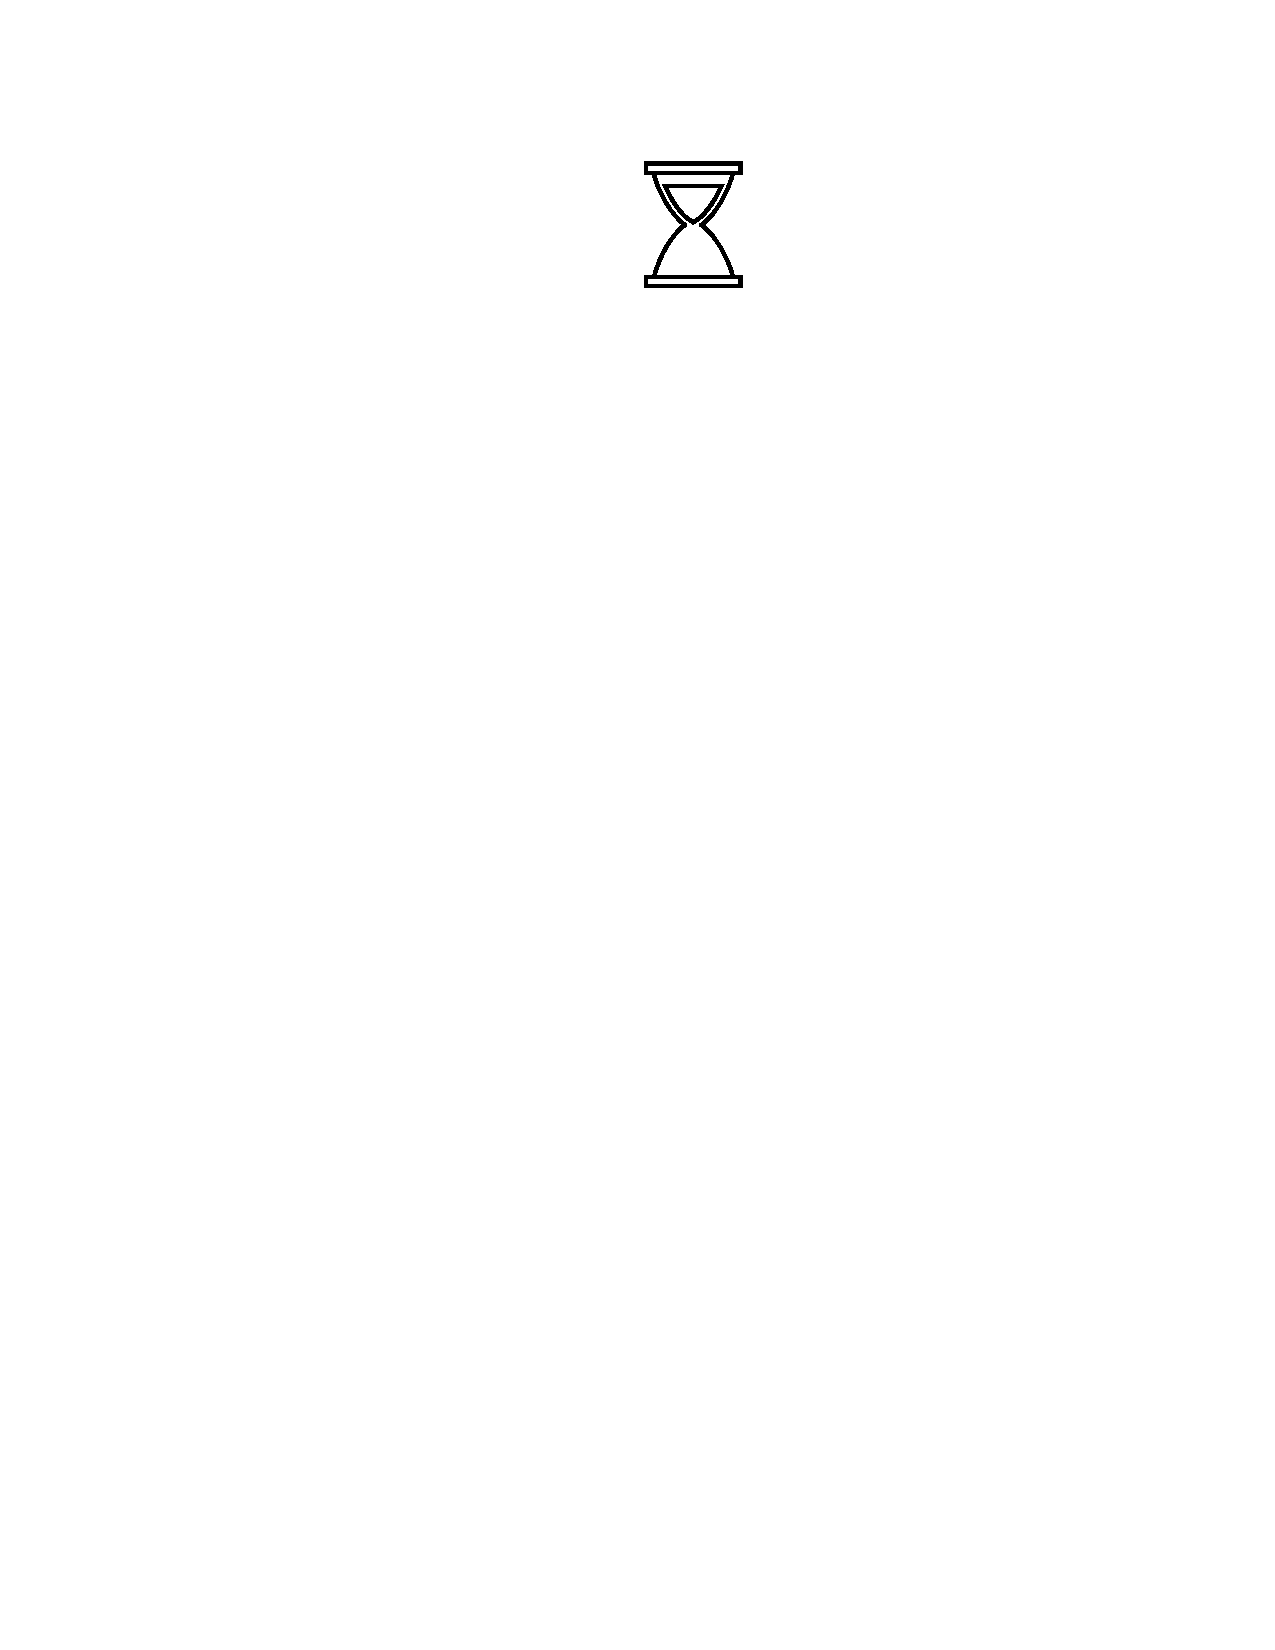
\includegraphics[width=\linewidth]{img/Risikotyp_Zeit}
\end{wrapfigure}

Vor dem Hintergrund, dass die Pilot-Phase eines Projekts per Definition der erstmaligen Erprobung risikobehafteter Entwicklungen dient, ist das Auftreten von Softwarefehlern sehr wahrscheinlich. Sollten die Großkunden den Druck auf die Geschäftsführung weiter erhöhen, ist es zudem möglich, dass die Testphase zugunsten einer frühen Auslieferung verkürzt wird, was Wahrscheinlichkeit für das Auftreten von Bugs maßgeblich erhöhen würde. Der Schaden, welcher hierdurch entstehen würde, ist nicht zu unterschätzen. Zum einen wird hierdurch eine Verlängerung des Projekts zur Behebung der Fehler nötig und zum anderen kann es einen erheblichen Imageschaden hervorrufen. Je nach Ausmaß der Anzahl und Größe der Softwarefehler, könnten die Kunden, welche ohnehin bereits unzufrieden mit der von uns erbrachten Leistung sind, sogar eine Kündigung in Betracht ziehen. Zwecks Verringerung der Eintrittswahrscheinlichkeit dieses Risikos werden folgende Maßnahmen ergriffen:
\begin{itemize}
	\item Die geplante Länge der Testphase ist zwingend einzuhalten. Auf Anfrage der Großkunden kommuniziert der Product Owner ihnen detailliert, welche Vorteile sich aus einem ausführlichen Testing für sie ergeben.
	\item Während der Entwicklungsphase werden robuste Unit-, Integration- und End-To-End-Tests implementiert und dokumentiert. Die Tests sind stets von dem Entwickler umzusetzen, welcher für die Realisation der entsprechende Funktionseinheit oder Schnittstelle verantwortlich ist. 
\end{itemize}